% recto + verso: dedication or epigraph
\newgeometry{left=19mm, right=80mm, top=6pc, bottom=6pc}
\thispagestyle{empty}
{
    \begin{fullwidth}
        \flushright{}
        \hfill 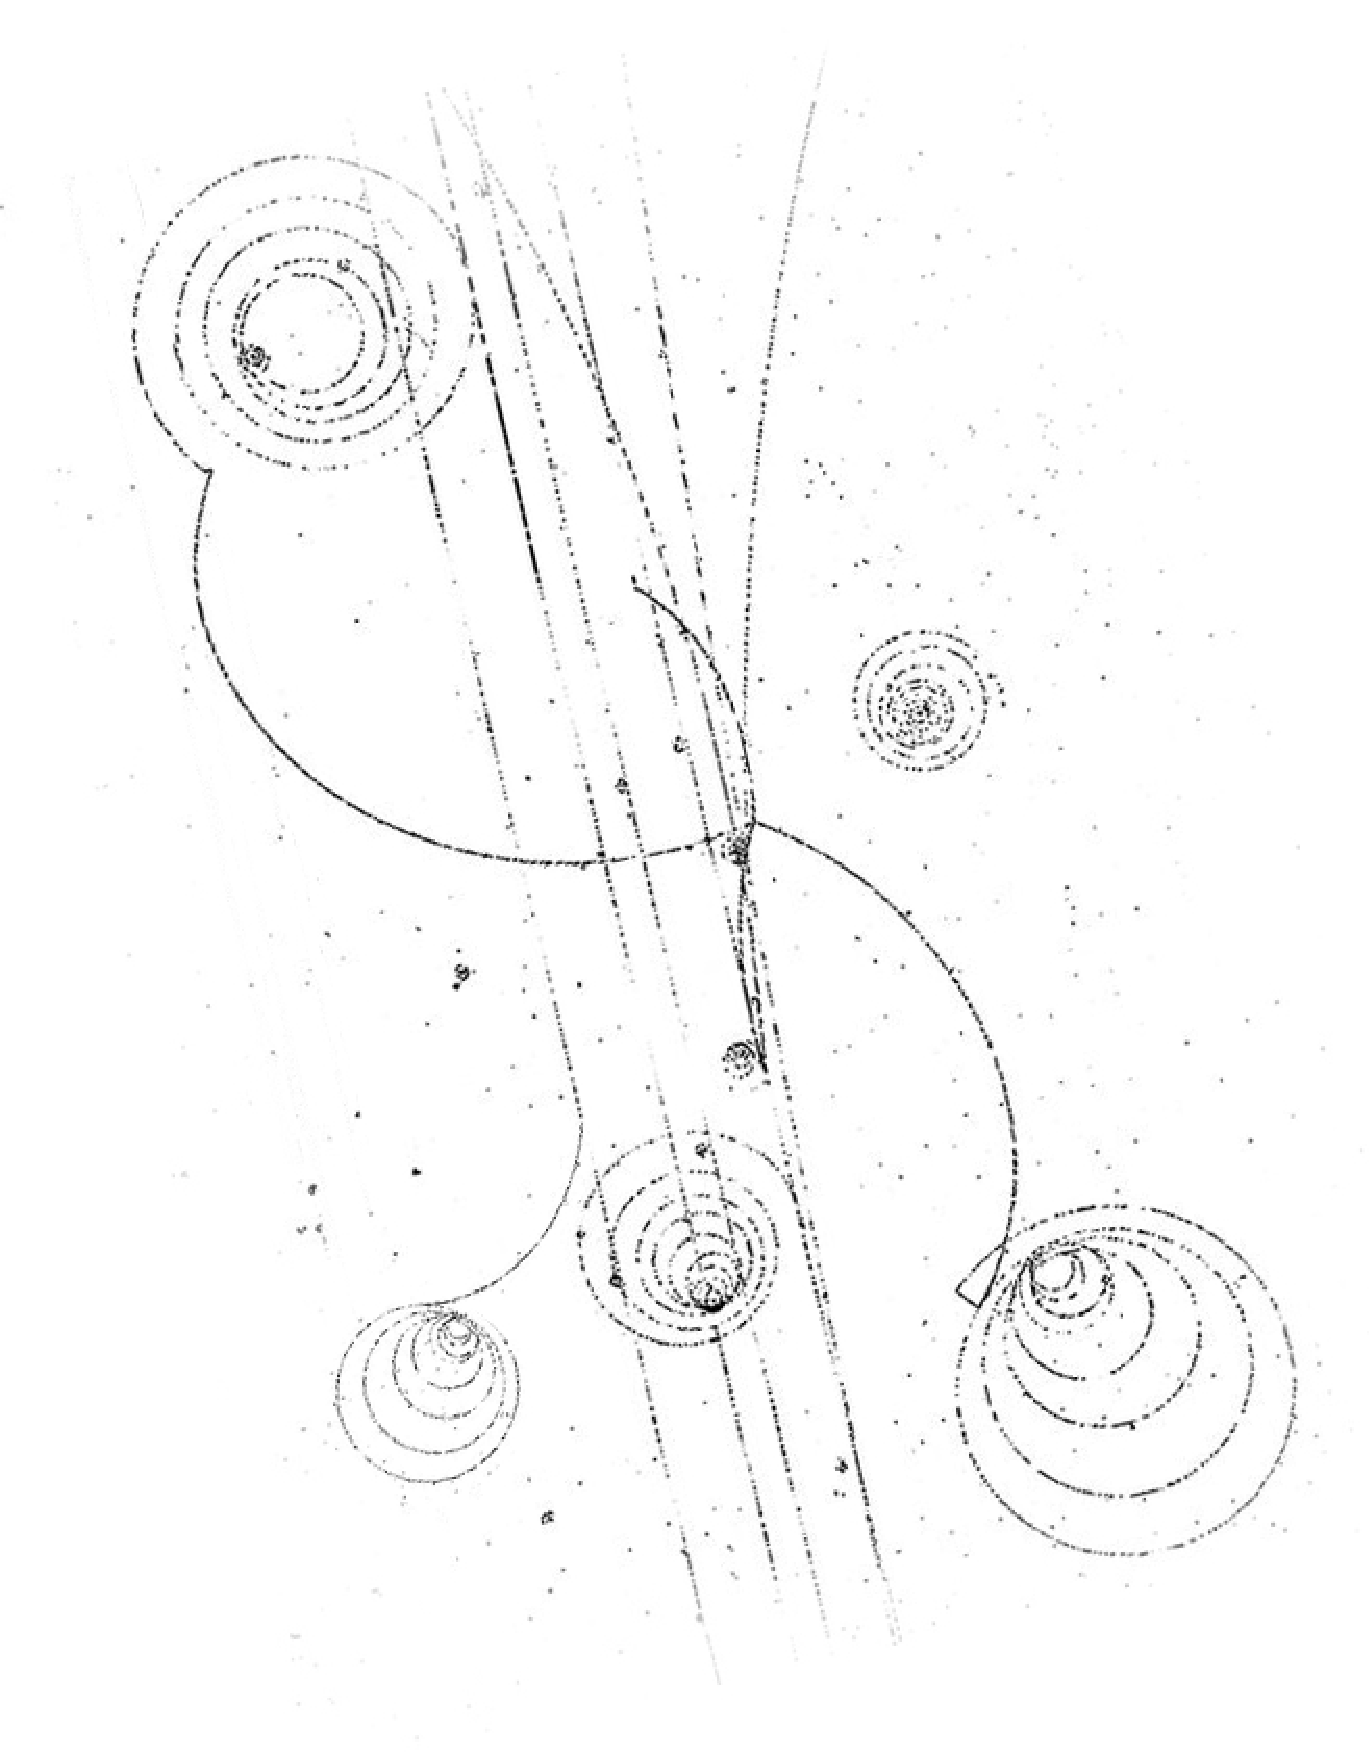
\includegraphics[width=\textwidth]{Assets/Images/Particle_tracks.pdf}
    \end{fullwidth}

    %\vfill

    \section*{\normalsize Agradecimientos}\addcontentsline{toc}{chapter}{Agradecimientos}

    A mis directores, Tere y Hernán, que me acompañaron y me guiaron en esta última hermosa etapa de la carrera, que desde que comencé había esperado con tantas ansias. Gracias por la dedicación, el tiempo, y la confianza en todo el muy agitado e imprevisible 2021. Gracias Tere por tus ``datos Billiken'' en FGIV, por los comentarios y las anécdotas de ATLAS al final de las clases, y por preocuparte y darme un lugar en el grupo cuando llegó el momento de comenzar\dots

    A Jose, con quién dí los primeros pasos para entrar en este increible e infinito mundo\dots

    To Nadav, Damiano and Liron, from the HEP group in Tel Aviv University. Thank you for all the suggestions, support, code-checking and late night answers through all these months\dots

    A mi Mamá, a mi Papá, a Cuerdi, y a toda mi familia. Gracias por haberme enseñado a ser quién soy, por el apoyo incondicional, por los valores, por responderme los ``porqués'' a las 11 de la noche cuando era chiquito, por los libros, por la compañia, por los tés y tortas de madrugada, por todos los abrazos, el amor, las palabras, y la paciencia\dots

    A Pedro, Tomi, Capu, Jose, Valen, los Enzos, Flor, Cande, Santi, y todas las increibles personas que conocí desde el primer día que traspasé las puertas de la Facultad, y que me llevo para toda la vida\dots

    A Juli, mi casi hermana, por acompañarme siempre en las risas, en las frustraciones, en las alegrías y en los enojos\dots

    A todos mis amigos de Quilmes, por siempre estar ahí aún con las semanas de desconexión\dots

    A mis Profesores, Jefes de Trabajos Prácticos y Ayudantes, de quienes no solo aprendí Física, sino integridad académica. Gracias especialmente a Fer, Claudia, Joe y Lisandro, quienes despertaron en los primeros años de mi carrera la curiodidad inacabable por la física experimental. Gracias también a Mauricio, por enseñarme a hacer cuentas y aproximaciones, y a Raúl, por introducirme al hermoso mundo de la Computación Cuántica, al que planeo también acudir durante mis próximos años de trabajo en HEP\dots

    Al proyecto arXiv\sidenote{\url{https://arxiv.org/}}, al SEDICI\sidenote{\url{http://sedici.unlp.edu.ar/}}, y a todos los repositorios de información científica abiertos y gratuitos, por permitir el acceso a la Ciencia a millones de personas en el mundo\dots

    To the increidible community at CERN, that made possible my participation in the Summer Programme during which part of this thesis was developed\dots
}

\cleardoublepage{}
